%==============================================================================
% Documentation (pdflatex --interaction=nonstopmode this_file.spad
% Note: ensure that the code above is between \iffalse ... \fi.
%==============================================================================
\documentclass[12pt,a4paper]{article}
\usepackage[utf8]{inputenc}
\usepackage[english]{babel}
\usepackage{amsmath}
\usepackage{amsfonts}
\usepackage{amssymb}
\usepackage{makeidx}
\usepackage{graphicx}
\usepackage{listings}
\usepackage{color}
\usepackage{epstopdf}

\definecolor{dkgreen}{rgb}{0,0.6,0}
\definecolor{gray}{rgb}{0.5,0.5,0.5}
\definecolor{mauve}{rgb}{0.58,0,0.82}
\definecolor{orange}{rgb}{1.0,0.44,0}

\lstdefinelanguage{SPAD}
{keywords={if,then,else,for,in,repeat},
keywords=[2]{Fraction,Integer,Polynomial,RealClosure,Cell, Float, 
             DoubleFloat, CylindricalAlgebraicDecompositionPackage, 
             List},
keywords=[3]{cylindricalDecomposition},
keywordstyle=[2]\color{red},
keywordstyle=[3]\color{orange},
sensitive=true,%
alsoletter={\$},%
comment=[l]{--},%
string=[b]",%
string=[b]'%
}

\lstset{frame=tb,
  language=SPAD,
  aboveskip=3mm,
  belowskip=3mm,
  showstringspaces=false,
  columns=flexible,
  basicstyle={\small\ttfamily},
  numbers=none,
  numberstyle=\tiny\color{gray},
  keywordstyle=\color{blue},
  commentstyle=\color{dkgreen},
  stringstyle=\color{mauve},
  breaklines=true,
  breakatwhitespace=true,
  tabsize=3
}
\author{Kurt Pagani \\ {\tt nilqed@gmail.com}}
\date{\today}
\title{DifferentialForms \\ {\small\tt FriCAS package:DFORM \\ Version 1.2}}
%
\newcommand{\CAD}{{\tt CAD}}
\newcommand{\QE}{{\tt QE}}
\newcommand{\RR}[1]{\mathbb{R}^{#1}}
\newcommand{\QQ}[1]{\mathbb{Q}^{#1}}
\newcommand{\ZZ}[1]{\mathbb{Z}^{#1}}
\newcommand{\KK}[1]{\mathbb{K}^{#1}}
\newcommand{\spadfun}[1]{\textcolor{magenta}{\tt #1}}
\newcommand{\spadbold}[1]{{\tt\bf #1}}
\newcommand{\type}[1]{\textcolor{blue}{\tt\tiny #1}}
\makeindex
\begin{document}
\maketitle
%
\begin{abstract}
Reference manual for the package {\tt DifferentialForms}.
\end{abstract}
%
\tableofcontents
%
\section{Introduction}
The package {\tt DifferentialForms} (file: {\tt dform.spad}) builds on the
domain {\tt DeRhamComplex}. In the following section we will give a brief 
overview of the functions that are going to be implemented. The focus is 
on precise definitions of the notions, since those may be varying in the 
literature. In section (2) we will describe the exported functions and 
how they work, in section (3) some short implementation notes will be 
given and finally the last section is devoted to some examples.
%
\section{Definitions}
Let ${\cal M}$ be a n-dimensional manifold (sufficiently smooth and orientable). 
To each point $P\in{\cal M}$ there is a neighborhood which can be 
diffeomorphically mapped to some region in $\RR n$, with coordinates
\begin{displaymath}
   x_1 (P'), \ldots, x_n (P')
\end{displaymath}
for all $P' \in \mathcal{U} (P) \subset \mathcal{M}$. The tangent space
$T_{P'} (\mathcal{M})$ at the point $P'$ is a vector space that 
is spanned by the basis
\begin{displaymath}
    e_1 (P'), \ldots, e_n (P')
\end{displaymath}
which also is often denoted by 
\begin{displaymath}
   \partial_1, \ldots, \partial_n =
   \frac{\partial}{\partial x_1}, \ldots, 
   \frac{\partial}{\partial x_n}.  
\end{displaymath}
A tangent vector $v$ has the form

\begin{displaymath}
  v = \sum_{j = 1}^n v^j e_j . 
\end{displaymath}
The cotangent space $T_{P'}^{} (\mathcal{M})^{\star}$ is the vector space
of linear functionals 
\begin{displaymath}
   \alpha : T_{P'} (\mathcal{M}) \rightarrow \mathbb{R},
\end{displaymath}
spanned by the basis $e^1 (P'), \ldots, e^n (P')$
which (corresponding to the basis $\partial_j$) is also denoted by 
\begin{displaymath}
	d x^1,\ldots, d x^n. 
\end{displaymath}
The latter notation indicates the dependency on the moving
point $P'$. The dual basis is by definition comprised of those linear
functionals such that
\begin{displaymath}
  e^j (e_k) = \delta^j_k . 
\end{displaymath}
Therefore we have 
\begin{displaymath}
	\alpha (v) = \alpha \left( \sum_{j = 1}^n v^j e_j \right) =
   \sum_{j = 1}^n v^j \alpha (e_j) = \sum_{j = 1}^n v^j \alpha_j,
\end{displaymath}
where $\alpha = \sum_{j = 1}^n \alpha_j e^j$.   

\subsection{Inner product of differential forms ({\tt dot})}
Let $g_x$ be a symmetric $n \times n$ matrix which is 
nondegenerate (i.e. $\det (g_x) \neq 0$). The index $x$ indicates that 
this matrix depends on the coordinates $x_1 (P), \ldots, x_n (P)$ and 
may be varying from point to point. If this dependency is smooth (enough) 
we speak of a (pseudo-) {\it Riemannian metric} (locally). This way we 
get an isomorphism between tangent vectors and $1$-forms (aka covectors):
\begin{displaymath}
	\alpha_j = g_{j k} v^k, \hspace{1.2em} v^j = g^{j k} \alpha_j .
\end{displaymath}
Clearly, $\sum_k g^{j k} g_{k l} = \delta^j_l$, in other words 
$(g^{j k})$ is the inverse of $g$. The metric $g$ defines an 
{\it inner product} on vectors,
\begin{displaymath}
	g (v, w) = \langle v, w \rangle : = g_{i j} v^i w^j 
\end{displaymath}
and by duality also on $1$-forms:
\begin{displaymath}
	 g^{- 1} (\alpha, \beta) = \langle \alpha, \beta \rangle : = g^{i j}
   \alpha_i \beta_j . 	
\end{displaymath}
Now, this inner product is extended to arbitrary $p$-forms by
\begin{displaymath}
	  \langle \alpha_1 \wedge \ldots \wedge \alpha_p , \beta_1 \wedge
  \ldots \wedge \beta_p \rangle : = \det (\langle \alpha_i, \beta_j \rangle)
  , \hspace{1.8em} (1 \leqslant i, j \leqslant p), \label{dot}
\end{displaymath}
and linearity.
%

\subsection{The volume form $\eta$ ({\tt volumeForm})}
The Riemannian {\it volume form} $\eta$ is (by definition) given by the 
$n$-form 
\begin{displaymath}
	 \eta = \sqrt{| \det g |} e^1 \wedge \ldots \wedge e^n = 
	 \sqrt{| \det\,g |} dx^1 \wedge \ldots \wedge d x^n . \label{vol}
\end{displaymath}
This definition makes sense because a (orientation preserving) change of
coordinates $\sqrt{\mathrm{det} g}$ transforms like the component of
a $n$-form.
%

\subsection{Hodge dual ({\tt hodgeStar})}
The {\it Hodge dual} of a differential $p$-form $\beta$ is the 
$(n - p)$-form $\star \beta$ such that
\begin{displaymath}
	 \alpha \wedge \star \beta = \langle \alpha, \beta \rangle \eta 
	 \label{hodge}
\end{displaymath}
holds, for all $p$-forms $\alpha$. The linear operator $(\star)$ is 
called the {\it Hodge star operator}. By the {\it Riesz representation
theorem} the Hodge dual is uniquely defined by the expression above.
%

\noindent
{\bf Warning:} {\it Flanders} \cite{FLAN} defines the Hodge dual by the 
equality
\begin{displaymath}
	 \lambda \wedge \mu = \langle \star \lambda, \mu \rangle \eta 
\end{displaymath}
where $\lambda$ is a $p$-form and $\mu$ a $(n-p)$-form.
This may result in different signs (actually $\star_F = s(g)\star$,
where $s(g)$ is the {\it sign} of the determinant of $g$).
 
The generally adopted definition is the one given at the beginning 
of this subsection. 

The components of $\star \beta$ are

\begin{displaymath}
	(\star \beta)_{j_1, \ldots, j_{n - p}} = \frac{1}{p!} \varepsilon_{i_1,
   \ldots, i_p, j_1, \ldots, j_{n - p}}  \sqrt{| \det g |} g^{i_1 k_1} \ldots
   g^{i_p k_p} \beta_{k_1, \ldots, k_p} 
\end{displaymath}
what is equal to
\begin{displaymath}
	 \frac{1}{p! \sqrt{| \det g |}} \varepsilon_{}^{k_1, \ldots, k_p, l_1,
   \ldots, l_{n - p}} g_{j_1 l_1} \ldots g_{j_{n - p}, l_{n - p}} \beta_{k_1,
   \ldots, k_p} .
\end{displaymath}
%

\subsection{Interior product $i_v$ ({\tt interiorProduct})}
The {\it interior product} of a vectorfield $v$ and a $p$-form $\alpha$
is a $(p-1)$-form $i_v(\alpha)$ such that
\begin{displaymath}
	 i_v (\alpha) (v_1, \ldots, v_{p - 1}) = 
	   \alpha (v, v_1, \ldots, v_{p - 1})
\end{displaymath}
holds for all vectorfields $`v_1, \ldots, v_{p - 1}$. Therefore, the 
components of $i_v (\alpha)$ are calculated to
\begin{displaymath}
	 i_v (\alpha)_{j_1, \ldots, j_{p - 1}} = 
	 v^j \alpha_{j, j_1, \ldots, j_{p -1}}.
\end{displaymath}
One can express the interior product by using the $\star$-operator. 
Let $\alpha$ be the $1$-form defined by the equation 
\begin{displaymath}
	 \alpha (w) = g (v, w), \forall w. 
\end{displaymath}
This means in components: $\alpha_j = g_{j k} v^k$, 
thus we have
\begin{displaymath}
	i_v (\beta) = (-)^{p - 1} \star^{- 1} (\alpha \wedge \star \beta) .
\end{displaymath}
Clearly, the interior product is independent of any metric, whereas the 
Hodge operator is {\bf not}! So, usually one should not use the Hodge 
operator to compute the interior product.

We will use the fact that the interior product is an {\it antiderivation},
which will allow a recursive implementation.
%

\subsection{The Lie derivative $\mathcal{L}_v$ ({\tt lieDerivative})} 
The {\it Lie derivative} with respect to a vector field $v$ can be 
calculated (and defined) using {\it Cartan's} formula:
\begin{displaymath}\label{cartan}
	\mathcal{L}_v \alpha = d i_v (\alpha) + i_v (d \alpha).
\end{displaymath}

There are other ways to define $\mathcal{L}_v \alpha$, however, 
it is convenient to compute it this way when $d$ and $i_v$ are 
already at hand.
%

\subsection{The CoDifferential $\delta$ ({\tt codifferential})}
The {\it codifferential} $\delta$ acting on a $p$-form is defined 
as follows:
\begin{displaymath}
	 \delta = (-1)^{n(p-1)+1}\,s(g) \star\,d\,\star
\end{displaymath}
where $g$ is the metric and $s(g)$ is related to the 
{\it signature} of $s(g)$ as described next.
%

\subsection{The sign of a metric  $s(g)$ ({\tt s})}
The signature of a metric $g$ is defined as the difference of
the number of positive ($p$) and negative ($q$) eigenvalues, i.e:
\begin{displaymath}
	\mathrm{signature(g)} = p - q
\end{displaymath}
and the {\it sign} function $s$ is defined as
\begin{displaymath}
	s(g) = (-1)^{\frac{n -\mathrm{signature(g)}}{2}} 
\end{displaymath}
Since we always assume that $g$ is non-degenerate, we have 
$p+q=n$, and consequently
\begin{displaymath}
	s(g) = (-1)^{q} = \mathrm{sign}\, \mathrm{det}(g)
\end{displaymath}
%

\subsection{The inverse Hodge star $\star^{-1}$ ({\tt invHodgeStar})}
Applying the Hodge star operator on a $p$-form twice we get
the identity map up to sign:
\begin{displaymath}
	\star\circ\star\, \omega_p = (-1)^{p(n-p)}\,s(g)\,\omega_p.
\end{displaymath}
Therefore
\begin{displaymath}
	\star^{-1}\,\omega_p = (-1)^{p(n-p)}\,s(g)\,\star\omega_p. 
\end{displaymath}
%

\subsection{The Hodge-Laplacian $\Delta_g$ ({\tt hodgeLaplacian})}
The {\it Hodge-Laplacian}, also known as {\it Laplace-de Rham operator} 
is defined on any manifold equipped with a (pseudo-) Riemannian
metric $g$ and is defined by
\begin{displaymath}
	\Delta_g = d\circ\delta + \delta\circ d
\end{displaymath}

Note that in the {\it Euclidean} case $\Delta_g = - \Delta$, where
latter is the ordinary {\it Laplacian}.
%
%
%
\section{Export}
%
\subsection{Package Details}
%

\begin{tabular}{|l|l|}
   \hline 
   {\bf Package Name:} & {\tt DifferentialForms} \\ 
   \hline 
   {\bf Abbreviation:} & {\tt DFORM} \\ 
   \hline 
   {\bf Source file(s):} & {\tt dform.spad} \\ 
   \hline 
   {\bf Dependent on} & {\tt DeRhamComplex (DERHAM)} \\ 
   \hline 
   \end{tabular}    
%
\begin{lstlisting}
    DifferentialForms(R,v) 
    
    R: Join(Ring,Comparable)     -- e.g. Integer
    v: List Symbol               -- e.g. [x,y,z] or [x[0],x[1],x[2]]

    X ==> Expression R           -- function Ring   
\end{lstlisting}
%
For the examples that follow we will choose {\tt R=Integer}, 
\begin{verbatim}
    v=[x[0],x[1],x[2],x[3]]},
\end{verbatim}
and the abbreviation {\tt M:=DFORM(R,v)}. Recall that indices of lists
and vectors in FriCAS start with $1$, so one has to be careful:
\begin{verbatim}
    v.1  -->  x[0].
\end{verbatim}
%

\subsection{The metric $g$}
Some functions expect the metric $g$ as a parameter. Generally this
will be provided by an invertible square matrix 
{\tt g:SquareMatrix(\#v,X)}. 
In the sequel we will choose the Minkowski metric:
%
\begin{lstlisting}    
    g := diagonalMatrix([-1,1,1,1])@SquareMatrix(4,Integer)
\end{lstlisting}   

\begin{displaymath}
	 \left[
  \begin{array}{cccc}
  -1 & 0 & 0 & 0 \\
  0 & 1 & 0 & 0 \\
  0 & 0 & 1 & 0 \\
  0 & 0 & 0 & 1
  \end{array}
  \right]
\end{displaymath}
%

\subsection{Exported functions}
The function \spadfun{baseForms} returns the basis one forms, while 
\spadfun{coordVector} returns a list of the coordinates. The function 
\spadfun{coordSymbols} also returns the coordinates, however, as symbols 
only (convenient when used with {\tt D}).
%
\begin{lstlisting} 
    
    SMR ==> SquareMatrix(#v,X)
    DRC ==> DeRhamComplex(R,v)

    dx:=baseForms()$M       -- [dx[0],...,dx[3]]
    x:=coordVector()$M      -- [x[0],...,x[3]]
    xs:=coordSymbols()$M    -- as above but as List Symbol 
                            -- e.g for differentiation D

\end{lstlisting} 
%
\subsubsection{Volume Form }
\spadbold{volumeForm}
  
Given a metric $g$ the function returns the corresponding volume 
element of the Riemannian (pseudo-) manifold.   

\begin{lstlisting}    
    volumeForm : SquareMatrix(#v,X) -> DeRhamComplex(R,v)    
    volumeForm(g)$M
\end{lstlisting}
\begin{displaymath}
	 {dx _ {0}} \  {dx _ {1}} \  {dx _ {2}} \  {dx _ {3}}	 
\end{displaymath}
\type{Type: DeRhamComplex(Integer,[x[0],x[1],x[2],x[3]])}
%
\subsubsection{Scalar Product} 
\spadbold{dot}

Compute the inner product of two differential forms with respect to the
metric $g$.
\begin{lstlisting}
    dot : (SMR,DRC,DRC) -> X    
    dot(g,dx.1*dx.2,dx.1*dx.2)$M   -- note dx.1 corresponds to dx[0].
\end{lstlisting}    
\begin{displaymath}
	-1
\end{displaymath}
\type{Type: Expression(Integer)}
%
\subsubsection{Hodge Star Operator}
\spadbold{hodgeStar}

Compute the Hodge dual form of a differential form with respect
to a metric $g$.
\begin{lstlisting}    
    hodgeStar : (SMR,DRC) -> DRC     
    hodgeStar(g,dx.2 * dx.3)    
\end{lstlisting} 
\begin{displaymath}
	{dx _ {0}} \  {dx _ {3}}
\end{displaymath}
\type{Type: DeRhamComplex(Integer,[x[0],x[1],x[2],x[3]])}
%
\subsubsection{Interior Product} 
\spadbold{interiorProduct}
  
Calculate the interior product $i_X(a)$ of the vector field $X$
with the differential form $a$.
\begin{lstlisting}
  interiorProduct : (Vector(X),DRC) -> DRC 
  interiorProduct(vector x, dx.1*dx.3)$M
\end{lstlisting}
\begin{displaymath}
	 {{x _ {0}} \  {dx _ {2}}} -{{x _ {2}} \  {dx _ {0}}}
\end{displaymath}
\type{Type: DeRhamComplex(Integer,[x[0],x[1],x[2],x[3]])}  
%
\subsubsection{Lie Derivative}
\spadbold{lieDerivative}
 
Calculate the Lie derivative $\mathcal{L}_X(a)$ of the differential 
form $a$ with respect to the vector field $X$.
\begin{lstlisting}    
    lieDerivative : (Vector(X),DRC) -> DRC   
    lieDerivative(vector x, dx.1 * dx.3 * dx.4)
\end{lstlisting}    
\begin{displaymath}
	3 \  {dx _ {0}} \  {dx _ {2}} \  {dx _ {3}}
\end{displaymath}
\type{Type: DeRhamComplex(Integer,[x[0],x[1],x[2],x[3]])}
%
\subsubsection{Co-differential}
\spadbold{codifferential}

Calculate the co-differential of a form with respect to a metric $g$.
\begin{lstlisting}
    codifferential(g,f*dx.1)$M 
\end{lstlisting}
%
\subsubsection{Sign of a metric $g$}
Calculate the  sign of a metric $g$.
\begin{lstlisting}
    s(g)
\end{lstlisting}
%
\subsubsection{Inverse Hodge star}
Calculate the inverse Hodge star operator:
\begin{lstlisting}
    invHodgeStar(g,dx.1)
\end{lstlisting}
%
\subsubsection{Hodge-Laplacian}
Calculate the Hodge-Laplacian.
\begin{lstlisting}
   hodgeLaplacian(g,f*dx.1)
\end{lstlisting}
%
\subsubsection{Projection}
\spadbold{proj}

Project to homogeneous terms of degree $p$.
  
\begin{lstlisting}
    NNI ==> NonNegativeInteger
    proj : (NNI,DRC) -> DRC    
    proj(2, 2*dx.1 + dx.2*dx.3 - dx.3*dx.4)
\end{lstlisting}
\begin{displaymath}
	 -{{dx _ {2}} \  {dx _ {3}}}+{{dx _ {1}} \  {dx _ {2}}}
\end{displaymath}
\type{Type: DeRhamComplex(Integer,[x[0],x[1],x[2],x[3]])}
%
\subsubsection{Monomials}
\spadbold{monomials}

List all monomials of degree $p$ ($p\in 1\ldots n$).
This is a basis of $\Lambda_p^n$.
\begin{lstlisting}
    monomials : NNI -> List DRC
    monomials(3)$M
\end{lstlisting}
\begin{displaymath}
  \left[
  {{dx _ {0}} \  {dx _ {1}} \  {dx _ {2}}}, \: {{dx _ {0}} \  {dx _
  {1}} \  {dx _ {3}}}, \: {{dx _ {0}} \  {dx _ {2}} \  {dx _ {3}}}, \:
  {{dx _ {1}} \  {dx _ {2}} \  {dx _ {3}}}
  \right]
\end{displaymath}
\type{Type: List DeRhamComplex(Integer,[x[0],x[1],x[2],x[3]])}
%
\subsubsection{Atomize Basis Term}
\spadbold{atomizeBasisTerm}

Given a basis term, return a list of the generators (atoms).
\begin{lstlisting}
    atomizeBasisTerm : DRC -> List DRC  
    atomizeBasisTerm(dx.1 * dx.2 * dx.4) 
\end{lstlisting}
\begin{displaymath}
  \left[
   {dx _ {0}}, \: {dx _ {1}}, \: {dx _ {3}}
  \right]
\end{displaymath}
\type{Type: List(DeRhamComplex(Integer,[x[0],x[1],x[2],x[3]]))}
%
\subsubsection{Conjugate Basis Term}
\spadbold{conjBasisTerm}

Return the complement of a basis term with respect to the Euclidean
volume form.
\begin{lstlisting}
    conjBasisTerm : DRC -> DRC    
    conjBasisTerm dx.4
\end{lstlisting}
\begin{displaymath}
	{dx _ {0}} \  {dx _ {1}} \  {dx _ {2}}
\end{displaymath}
\type{Type: DeRhamComplex(Integer,[x[0],x[1],x[2],x[3]])}
%
\subsubsection{Scalar and Vector Field} 
\spadbold{vectorField}

Generate a generic vector field named by a given symbol.
\\
\spadbold{covectorField}

Generate a generic co-vector field named by a given symbol.
\\  
\spadbold{scalarField}

Generate a generic scalar field named by a given symbol.
\begin{lstlisting}
   vectorField   : Symbol -> List X
   covectorField : Symbol -> List DRC
   scalarField   : Symbol -> X
   
   vectorField(Q)$M
   scalarField(f)$M
\end{lstlisting}
\begin{displaymath}
	[Q_1(x_0,x_1,x_2,x_3),Q_2,Q_3,Q_4]
\end{displaymath}
\type{Type: List(Expression(Integer))}
%
\begin{displaymath}
	 f
  \left(
   {{x _ {0}}, \: {x _ {1}}, \: {x _ {2}}, \: {x _ {3}}}
  \right)
\end{displaymath}
\type{ype: Expression(Integer)}
%
\subsubsection{Miscellaneous Functions}
A {\it zero form} with symbol $s$ can be generated by
\begin{lstlisting}
    zeroForm : Symbol -> DRC  
    zeroForm(s)$M
\end{lstlisting}
\begin{displaymath}
	  s
  \left(
   {{x _ {0}}, \: {x _ {1}}, \: {x _ {2}}, \: {x _ {3}}}
  \right)
\end{displaymath}
\type{Type: DeRhamComplex(Integer,[x[0],x[1],x[2],x[3]])}
%

A synonym for the \spadfun{exteriorDerivative} is the common operator 
\spadbold{d}:
\begin{lstlisting}
    d : DRC -> DRC    
    d zeroForm(f)$M
\end{lstlisting}
\begin{displaymath}
   f,_{4} dx_3 + \ldots +  f,_{1} dx_0
\end{displaymath}
\type{Type: DeRhamComplex(Integer,[x[0],x[1],x[2],x[3]])}
\\
{\bf Notice} the indices in the example above. We have deliberately 
chosen $0$ as start value to see where one has to be cautious. The
derivatives of the function $f$, for instance $f,_{4}$, are meant
with respect to the order of the variables, $x_3$ in this case. 
%

The special zero forms \spadbold{0} and \spadbold{1} can be generated 
by
\begin{lstlisting}
    one :  -> DRC
    zero : -> DRC    
    zero()$M
    one()$M
\end{lstlisting}
There are also some special multiplication operators which allow to deal
with a kind {\it vector valued} forms (actually lists):
\begin{lstlisting}
    _* : (List X, List DRC)   -> DRC
    _* : (List DRC, List DRC) -> DRC
    Note: the lists must have dimension #v.    
    For instance:   
    x * dx 
\end{lstlisting}
\begin{displaymath}
 {{x_{3}} \  {dx_{3}}}+{{x_{2}} \  {dx_{2}}}+{{x_{1}} \
  {dx_{1}}}+{{x_{0}} \ {d _{0}}}  
\end{displaymath}
%
An example for the second case:
\begin{lstlisting}
    dx*[hodgeStar(g,dx.j)$M for j in 1..4]
\end{lstlisting}
\begin{displaymath}
    2 \  {dx _ {0}} \  {dx _ {1}} \  {dx _ {2}} \  {dx _ {3}}
\end{displaymath}
\type{Type: DeRhamComplex(Integer,[x[0],x[1],x[2],x[3]])}
%
%
%
\section{Implementation}
\subsection{Implementation Notes} 
In this section some implementation details will be described. This is a 
ongoing process and might be improved.
\subsection{Internal Representation}
Differential forms are represented as {\tt List Record(k:EAB, c:R)} 
where each basic term is represented as {\tt Record(k:EAB, c:R)}, 
for instance:
\begin{displaymath}
  h (x, y, z)\ dz + g (x, y, z)\ dy + f (x, y, z)\ dx
\end{displaymath}
maps to
\begin{lstlisting}
    [[k= [0,0,1],c= h(x,y,z)],[k= [0,1,0],c= g(x,y,z)],
     [k= [1,0,0],c= f(x,y,z)]]
\end{lstlisting}
or, another example:
\begin{displaymath}
 c (x, y, z)\ dy\ dz + b (x, y, z)\ dx\ dz + a (x, y, z)\ dx\ dy
\end{displaymath}
goes to
\begin{lstlisting}
    [[k= [0,1,1],c= c(x,y,z)],[k= [1,0,1],c= b(x,y,z)],
     [k= [1,1,0],c= a(x,y,z)]]
\end{lstlisting}
It is easily seen that for n generators $x_1, \ldots, x_n$ the term 
$d x_{j_p} \wedge \ldots \wedge d x_{j_q}$ is represented by
$\mathtt{[k = [a_{i_1}, \ldots, a_{i_n}], c = \pm 1]}$
where $a_{i_s} \in \{ 0, 1 \}$ depending on whether 
$d x_{i_s}$ is contained in the term or not. The (local) function 
 {\bf terms} send a differential form $\omega$ to the representation 
$r(\omega)$.
Note that the operations are {\bf destructive}, this means that one has 
to copy the objects in order to get new ones (mere assignment inherits 
all previous changes).

The interpreter normalizes the basic terms according to increasing
generators, i.e for example: $d x_3 \wedge d x_2$ will be stored 
as $- d x_2 \wedge d x_3$, whereby the signum of the permutation is 
calculated and transferred to the $c$-field in the record.
\begin{lstlisting}
Example
  
    terms(dx3*dx2) -> [[k= [0,1,1],c= - 1]]
\end{lstlisting}
%
\subsection{dot :: inner product}
Given a (pseudo)-Riemannian metric $g$, the scalar product of two basic 
terms of the same degree is given by
\begin{displaymath}
 \langle d x_{i_1} \ldots d x_{i_p}, d x_{j_1} \ldots d x_{j_p} \rangle =
   \det (\langle d x_{i_k} , d x_{j_l} \rangle) = \det (g^{- 1} (i_k,
   j_l)),
\end{displaymath}
whereby $1 \leqslant k, l \leqslant p$. Note that 
$g^{- 1} (i_k, j_l) = g^{i_k j_l}$ is the inverse of 
$g_{i_k j_l}$ (raised indexes as usual). In other words, the scalar 
product is inherited from the dual vector space of the space where the 
coordinates $(x_1, \ldots, x_n)$ live, and is continued by linearity.
By the way, terms of different \spadbold{degree} are considered to be
{\it orthogonal} to each other.
\begin{lstlisting}
Example
  
    [x,y,z], G = matrix(G[i,j]) = g^{- 1}
\end{lstlisting}
\begin{displaymath}
\langle d x \wedge d y, d y \wedge d z \rangle = \langle d x, d y \rangle
     \langle d y, d z \rangle - \langle d x, d z \rangle \langle d y, d y
     \rangle = \\ {G_{1,2} G_{2, 3} - G_{1, 3} G_{2, 2}} 
\end{displaymath}
The corresponding {\tt EAB's} are {\tt [1,1,0]} and {\tt [0,1,1]}. 
When we define a function \spadfun{pos} which gives the positions of 
$0$ or $1$ respectively, the example above tells us:
\begin{lstlisting}
    pos([1,1,0],1)=[1,2] and pos([0,1,1],1)=[2,3]
\end{lstlisting}
so that the direct product of the two resulting lists gives the desired 
minor:
\begin{lstlisting}
     [1,2]x[2,3]=[[1,2],[1,3],[2,2],[2,3]] =>
\end{lstlisting}
\begin{displaymath}
  \left|\begin{array}{c}
     G_{12} G_{1 3}\\
     G_{2 2} G_{2 3}
   \end{array}\right| .
\end{displaymath}
This essentially comprises the method we will use to compute the scalar 
product w.r.t symmetric matrices $g$ and two basic terms of equal degree.

\noindent Local function: \spadbold{dot2}
\begin{itemize}
\item compute the inverse of {\tt g}.
\item build the {\tt pos} lists.
\item build the minor and apply \spadfun{determinant}.
\end{itemize}
Actually there are two functions \spadbold{dot1} and \spadbold{dot2}, 
where the former is used when the metric $g$ is {\it diagonal} 
(which is equivalent to the basis vectors being orthogonal) because 
the performance might be better if the dimension of the space is huge.
%
\subsection{hodgeStar :: Hodge dual}
In this new version we have removed the first method because the
performance difference is not as significant as we thought in the first
place, at least not for $n\leq 7$. However, we save the method in
case someone has to deal with really high space dimensions.
\subsubsection{Diagonal, non-degenerated $g$}
If g is a diagonal matrix then the components of $\star \beta$ reduce to
\begin{displaymath}
(\star \beta)_{j_1, \ldots, j_{n - p}} = \frac{1}{p!} \varepsilon_{k_1,
   \ldots, k_p, j_1, \ldots, j_{n - p}}  \sqrt{| \det g |}  [g^{k_1 k_1}
   \ldots g^{k_p k_p}] \beta_{k_1, \ldots, k_p} 
\end{displaymath}
which implies that $(j_1, \ldots, j_{n - p})$ must be the complement of 
$(k_1,\ldots, k_p)$ in $\{ 1, 2, \ldots, n \}$ and
\begin{displaymath}
  \star (d x_{k_1} \wedge \ldots \wedge d x_{k_p}) = C d x_{j_1} \wedge
   \ldots \wedge d x_{j_{n - p}} 
\end{displaymath}  
for some (yet unknown) factor {\tt C} which must actually be equal to 
the right hand side of the component formula above. When we recollect 
the internal representation of $d x_{k_1} \wedge \ldots \wedge d x_{k_p}$ 
as {\tt EAB} then it is easy to get the complement by flipping
$0$ and $1$. Define a function \spadfun{flip} such that
\begin{displaymath}
  \mathrm{flip} (d x_{k_1} \wedge \ldots \wedge d x_{k_p}) = d x_{j_1} 
  \wedge \ldots \wedge d x_{j_{n - p}}
\end{displaymath}
then by using the Hodge formula with 
$\alpha = \beta = dx_{k_1} \wedge \ldots \wedge d x_{k_p}$ we get using
$\star \alpha = C\ \mathrm{flip} (\alpha)$:
\begin{displaymath}
  C \alpha \wedge \mathrm{flip} (\alpha) = \langle \alpha, \alpha 
  \rangle \eta
   = \langle \alpha, \alpha \rangle \sqrt{| \det (g) |} d x_1 \wedge 
   \ldots\wedge d x_n . 
\end{displaymath}
Since $\alpha \wedge \mathrm{flip} (\alpha)$ is a $n$-form, the function
\spadbold{leadingCoefficient} returns the one and only coefficient. 
Thus we can calculate {\tt C} to
\begin{displaymath}
  C = \frac{\langle \alpha, \alpha \rangle \sqrt{| \det (g)
   |}}{\mathtt{leadingCoefficient} (\alpha \wedge \mathrm{flip} (\alpha))}.
\end{displaymath}
In {\tt SPAD} syntax this looks like:
\begin{displaymath}
 \mathtt{C =}  \frac{\mathtt{dot} (\alpha, \alpha) \star
   \mathtt{sqrt\left(abs\left(\right.determinant\left(g\right)\right)}}
   {\mathtt{leadingCoefficient}
   \left( \alpha \star \mathtt{flip} (\alpha) \right)} .    
\end{displaymath}
This way the interpreter saved us the tedious computation of the permutation
signatures. Moreover, we have not to care whether the metric $g$ is 
positive or negative definite.
%
\subsubsection{General case}
Let $J$ denote an ordered multi-index and $J_\sharp$ its dual.
Then a generic $p$-vector may be written as
\begin{displaymath}
   \beta = \sum_{|J|=p} b^J \ e_J.
\end{displaymath}
Thus by definition we obtain:
\begin{displaymath}
    \alpha\wedge\star\beta=(\alpha,\beta)\,\eta \Rightarrow
    e_J\wedge\star\beta=(e_J,\beta)\,\eta
\end{displaymath}
Since $\star\beta$ is a $(n-p)$-form, we get:
\begin{displaymath}
 \star\beta=\sum_{|K|=n-p} a^K e_K \Rightarrow
   \sum_{|K|=n-p} a^K e_J\wedge e_K=\sum_{|I|=p} b^I (e_J,e_I)=
   \sum_{|I|=p} g_{JI} b^I \eta = b_J \eta. 
\end{displaymath}
Now the term $e_J\wedge e_K$ is non-zero only if $K=J_\sharp$,
therefore
\begin{displaymath}
  a^{J_\sharp} =\sqrt{g}\, \epsilon(J)\, \sum_{|I|=p} g_{JI} b^I
\end{displaymath}
where $e_J\wedge e_{J_\sharp}=\epsilon(J)\, \eta\ $ defines 
$\epsilon$.

If we choose $\beta=e_M$ we finally get
\begin{displaymath}
  \star e_M = \sqrt{g} \sum_{|J|=p} \epsilon(J)\, g_{JM}\, e_{J_\sharp}.
\end{displaymath}
This formula will be used to compute the Hodge dual for {\it monomials}. 
We define a function \spadbold{hodgeBT}, in pseudo-code:
\begin{lstlisting}
    hodgeStarBT(dx[M])= sqrt(g)* 
       SUM[J] {eps(dx[J])*dot(g,dx[J],dx[M])*conjBasisTerm(dx[j])}
\end{lstlisting}
which then will allow computing the Hodge dual of any form by simple recursion:
\begin{lstlisting}
    hodgeStar(g:SMR,x:DRC):DRC ==
      x=0$DRC => x
      leadingCoefficient(x) * hodgeStarBT(g,leadingBasisTerm(x)) + _
        hodgeStar(g, reductum(x))
\end{lstlisting}
%
\subsubsection{interiorProduct :: Interior product}
In this newer version we have replaced the method which uses the Hodge
operator. Instead we used the fact that the interior product is 
an {\it antiderivation}, actually the unique antiderivation of degree 
$-1$ on the exterior algebra such that $i_X(\alpha)=\alpha(X)$:
\begin{displaymath}
      i_X(\beta\wedge\gamma)=i_X(\beta)\wedge\gamma)+
     (-1)^{{\mathtt deg}\, \beta}\ \beta\wedge i_X(\gamma)
\end{displaymath}
This also allows an easy implementation by recursion.
%
\subsubsection{lieDerivative :: Lie derivative}
Here we use {\it Cartan's formula} (see \ref{cartan}), so that there is 
not much more to say here.
\begin{lstlisting}
    lieDerivative(w:Vector X,x:DRC):DRC ==
      a := exteriorDifferential(interiorProduct(w,x))
      b := interiorProduct(w, exteriorDifferential(x))
      a+b
\end{lstlisting}
%
\subsubsection{proj :: Projection}
Since the elements of $\mathtt{DeRhamComplex}$ are in
\begin{displaymath}
  X = \bigoplus_{p = 0}^n \Omega^p (V) 
\end{displaymath}
it is convenient to have a function 
$\mathtt{proj}:\{ 0, \ldots,n \}\times X \rightarrow X$ which 
returns the projection on the homogeneous component
$\Omega^p (V)$. The implementation is straightforward when using the
internals of {\tt EAB}. Probably there are better ways to do this,
especially by using exported functions only.
\begin{lstlisting}
    ** deprecated **
    proj(x,p) ==
      t:List REA := x::List REA
      idx := [j for j in 1..#t | #pos(t.j.k,1)=p]
      s := [copy(t.j) for j in idx::List(NNI)]
      convert(s)$DRC
\end{lstlisting}
{\bf NEW:}In the new version we actually replaced the function above by 
the following recursive one:
\begin{lstlisting}
    proj(p,x) ==
      x=0 => x
      homogeneous? x and degree(x)=p => x
      a:=leadingBasisTerm(x)
      if degree(a)=p then
        leadingCoefficient(x)*a + proj(p, reductum x)
      else
        proj(p, reductum x)
\end{lstlisting}
{\bf Note} \\
We have changed the order of arguments from 
{\tt (DRC,NNI)} to {\tt (NNI,DRC)} because this corresponds more to the 
usual nomenclature of projections.
%
\section{Usage}
\subsection{Examples}
In this section we will give various examples.
\subsection{Calculus in $\RR 3$}
We will prove the following identities (see the summary %\ref{•}, for 
details):
\begin{eqnarray*}
    d\,f &= [\mathtt{grad}\,f]_1 \\
    d\,[T]_1 &= [\mathtt{curl}\,T]_2 \\
    d\,[T]_2 &= [\mathtt{div}\,T]_3
\end{eqnarray*}
Let M denote our differential graded algebra on $\RR 3$. In
{\tt FriCAS} we can express this as
\begin{lstlisting}
     M ==> DFORM(INT,[x,y,z])
\end{lstlisting}
\begin{displaymath}
  \mathtt{DifferentialForms(Integer,[x,y,z])}
\end{displaymath}
\type{Type: Type}
\\
The list of available methods can be seen by
\begin{lstlisting}
    )show M
    
    DifferentialForms(Integer,[x,y,z]) is a package constructor.
    Abbreviation for DifferentialForms is DFORM
    This constructor is exposed in this frame.
    ------------------------------- Operations -----------------

    coordSymbols : () -> List(Symbol)
    ...
    baseForms : () -> List(DeRhamComplex(Integer,[x,y,z]))
    coordVector : () -> List(Expression(Integer))
    .
    .
    .
\end{lstlisting}
The position vector $P=(x,y,z)$ and the basis of one forms can be
obtained by
\begin{lstlisting}
    P:=coordVector()$M
\end{lstlisting}
\begin{displaymath}
    [x,y,z]
\end{displaymath}
\type{Type: List(Expression(Integer))}
\\
and
\begin{lstlisting}
    dP:=baseForms()$M
\end{lstlisting}
\begin{displaymath}
  [dx,dy,dz]
\end{displaymath}
\type{Type: List(DeRhamComplex(Integer,[x,y,z]))}

This way we can call the coordinates as $P.i$ and the basis one forms
as $dP.i$. Of course, we can also use $dx,dy,dz$ directly when
setting
\begin{lstlisting}
     [dx,dy,dz]:=baseForms()$M
\end{lstlisting}
or when we use the generators of the domain {\tt DeRhamComplex} itself:
\begin{lstlisting}   
     dx:=generator(1)$DERHAM(INT,[x,y,z])
     dy:= ...    
\end{lstlisting}

The first method, however, is quite convenient when using indexed coordinates
and also because we can form expressions like
\begin{lstlisting}
    P * dP
\end{lstlisting}
\begin{displaymath}
   z\ dz + y\ dy + x\ dx
\end{displaymath}
\type{Type: DeRhamComplex(Integer,[x,y,z])}.
%
\subsubsection{Gradient} 
There are many ways to create a zero form, one of those is
\begin{lstlisting}
    f := zeroForm(f)$M
\end{lstlisting}
\begin{displaymath}
   f(x,y,z)
\end{displaymath}
\type{Type: DeRhamComplex(Integer,[x,y,z])}
\\
Now we apply the exterior differential operator to $f$:
\begin{lstlisting}
    d f
\end{lstlisting}
\begin{displaymath}
   {{{f _ {{,3}}}\left(
   {x, \: y, \: z}\right)}
   \  dz}+{{{f _ {{,2}}}\left({x, \: y, \: z}
   \right)}\  dy}+{{{f _ {{,1}}}
   \left({x, \: y, \: z}\right)}\  dx}
\end{displaymath}
\type{Type: DeRhamComplex(Integer,[x,y,z])}
\\
The coefficients of $df$ are just
\begin{lstlisting}
    [coefficient(d f, dP.j) for j in 1..3]
\end{lstlisting}
\begin{displaymath}
  \left[{{f _ {{,1}}}\left({x, \: y, \: z}
  \right)},\: {{f _ {{,2}}}\left(
  {x, \: y, \: z}\right)},
  \: {{f _ {{,3}}}\left({x, \: y, \: z}\right)}\right]
\end{displaymath}
\type{Type: List(Expression(Integer))}
\\ 
the components of the gradient vector $\nabla f$ of $f$.
%
\subsubsection{Curl}
Let $T$ be a generic vector field on $M=\RR 3$:
\begin{lstlisting}
    T := vectorField(T)$M
\end{lstlisting}
\begin{displaymath}
    \left[{{T _ {1}}\left({x, \: y, \: z}\right)},\: {{T _ {2}}
    \left({x, \: y, \: z}\right)},\: {{T _ {3}}\left({x, \: y, \: z}
    \right)}\right]
\end{displaymath}
\type{Type: List(Expression(Integer))}
\\
Then we build the general one form $\tau$:
\begin{lstlisting}
    tau := T * dP
\end{lstlisting}
\begin{displaymath}
    T_3\left(x, \: y, \: z\right)\  dz+T_2
   \left({x, \: y, \: z}
   \right)\  dy+T_1\left({x, \: y, \: z}\right)\  dx
\end{displaymath}

Now we apply the exterior differential operator $d$:
\begin{lstlisting}
    d tau
\end{lstlisting}
\begin{displaymath}
    \left( T_{3,2}\left(x, \: y, \: z\right)
    -T_{2,3}\left(x, \: y, \: z\right)\right)
    \ dy \ dz + \ldots
\end{displaymath}
\type{Type: DeRhamComplex(Integer,[x,y,z])}
\\
Next, we want to extract the coefficients:
\begin{lstlisting}
    [coefficient(d tau, m) for m in monomials(2)$M]
\end{lstlisting}
\begin{displaymath}
\scriptstyle{
    \left[{{{{T _ {2}} _ {{,1}}}\left({x, \: y, \: z}\right)}
    -{{{T _ {1}} _ {{,2}}}\left( {x, \: y, \: z}\right)}},
    \: {{{{T _ {3}} _ {{,1}}}\left({x, \: y, \: z}\right)}
    -{{{T _ {1}} _ {{,3}}}\left({x, \: y, \: z}\right)}},
    \: {{{{T _ {3}} _ {{,2}}}\left({x, \: y, \: z}
    \right)} -{{{T _ {2}} _ {{,3}}}\left({x, \: y, \: z}\right)}}
    \right]}
\end{displaymath}
\\    
The (well known) {\tt\bf curl} is defined as
\begin{displaymath}
    \mathtt{curl}(T) =\nabla\times T= \scriptstyle{
    \left(
    \frac{\partial T_3}{\partial y} - \frac{\partial T_2}{\partial z},
    \frac{\partial T_1}{\partial z} - \frac{\partial T_3}{\partial x},
    \frac{\partial T_2}{\partial x} - \frac{\partial T_1}{\partial y}
    \right)}
\end{displaymath}
\begin{lstlisting}
    curl(V) == [D(V.3,y)-D(V.2,z),D(V.1,z)-D(V.3,x),D(V.2,x)-D(V.1,y)]
\end{lstlisting}
We now claim that the following identity holds:
\begin{displaymath}
     d (T\, dP) =  \star(\mathtt{curl}(V)\, dP)
\end{displaymath}
where $\star$ denotes the Hodge star operator with respect to the Euclidean
metric
\begin{lstlisting}
    g:=diagonalMatrix([1,1,1])
\end{lstlisting}
\begin{displaymath}
   \left[
   \begin{array}{ccc}
   1 & 0 & 0 \\
   0 & 1 & 0 \\
   0 & 0 & 1
   \end{array}
   \right]
\end{displaymath}
To prove it we just have to test:
\begin{lstlisting}
     test( d(T*dP) = hodgeStar(g,curl(T)*dP)$M )
\end{lstlisting}
\begin{displaymath}
    \mathtt{true}
\end{displaymath}
\type{Type: Boolean}
%
\subsubsection{Divergence} 
Again, let $T$ be a generic vector field on $M={\RR 3}$, then the
{\it divergence} is defined by
\begin{displaymath}
   \mathtt{div}(T) = \nabla \bullet T =
   \frac{\partial T_1}{\partial x} +
   \frac{\partial T_2}{\partial y} +
   \frac{\partial T_3}{\partial z}.
\end{displaymath}
When we calculate
\begin{lstlisting}
    d hodgeStar(g, T*dP)$M
\end{lstlisting}
we get the 3-form
\begin{displaymath}
    {\left( {{{T _ {3}} _ {{,3}}}
    \left({x, \: y, \: z}\right)}+{{{T_ {2}} _ {{,2}}}
    \left({x, \: y, \: z}\right)}+{{{T_ {1}} _ {{,1}}}
    \left({x, \: y, \: z}\right)}\right)}\  dx \  dy \  dz
\end{displaymath}
%
\subsubsection{Summary}\label{summvc}
Let us summarize what we have obtained above. We use the following notation
for the mapping of scalar functions and vector fields to differential forms:
\begin{eqnarray*}
    f \rightarrow [f]_0 \\
    T \rightarrow [T]_1 
\end{eqnarray*}
where the index denotes the degree of the form. Moreover, we define another
pair of forms by applying the Hodge operator:
\begin{eqnarray*}
    [T]_2 &= \star [T]_1 \\
    \left[f\right[_3 &= \star [f]_0
\end{eqnarray*}
So we can state the general identities:
\begin{eqnarray*}
    d\,f &= [\nabla\,f]_1 \\
    d\,[T]_1 &= [\mathtt{curl}\,T]_2 \\
    d\,[T]_2 &= [\mathtt{div}\,T]_3
\end{eqnarray*}
%
\subsubsection{Hodge duals}
To conclude this example, we are going to calculate a table for the Hodge
duals of the monomials.
\begin{lstlisting}
     g:=diagonalMatrix([1,1,1])::SquareMatrix(3,INT) 
     [[hodgeStar(g,m)$M for m in monomials(j)$M] for j in 0..3]
     
\end{lstlisting}
\begin{displaymath}
   \left[{\left[ {dx \  dy \  dz}\right]},
   \: {\left[ {dy \  dz}, \: -{dx \  dz}, \: {dx \  dy}\right]},
   \: {\left[ dz, \: -dy, \: dx\right]},\: {\left[ 1\right]}\right]
\end{displaymath}
\type{Type: List(List(DeRhamComplex(Integer,[x,y,z])))}
\\
Thus we get the following table:
\begin{center}
\begin{tabular}{|c|c|c|}
\hline 
$\alpha$ & $\star\alpha$ & $\star\star\alpha$ \\ 
\hline 
$1$ & $dx\wedge dy \wedge dz$ & $1$ \\ 
\hline 
$dx$ & $dy \wedge dz$ & $dx$ \\ 
\hline 
$dy$ & $-dx \wedge dz$ & $dy$ \\ 
\hline 
$dz$ & $dx \wedge dy$ & $dz$ \\ 
\hline 
\end{tabular} 
\end{center}
By the way, this method can be applied in any dimension for any metric.
%
\subsection{Faraday $2$-form} 
The free electromagnetic field can be described by a $2$-form 
\spadbold{F} in Minkowski space. This form - also known as Faraday $2$-form - 
is given by
\begin{displaymath}
   %\scriptstyle{
   F=B_1\ dy\wedge dz + B_2\ dz\wedge dx + B_3\ dx\wedge dy +
     E_1\ dx\wedge dt + E_2\ dy\wedge dt + E_3\ dz\wedge dt 
   %}
\end{displaymath}
where we here use the {\it cgs} system and \spadbold{E},
\spadbold{B} denote the classical fields (see the example in the 
documentation of {tt DeRhamComplex}).

To represent \spadbold{F} in {\tt FriCAS} we have to choose space-time 
variables $x,y,z,t$ in the correct order, and $g$ will be the 
Minkowski metric:
\begin{lstlisting}    
    v := [x,y,z,t]   
    g := diagonalMatrix([-1,-1,-1,1])::SquareMatrix(4,INT)   
    M := DFORM(INT,v)    
    R ==> EXPR(INT)  
\end{lstlisting}

Instead of $x,y,z,t$ we also could have chosen $x_0,x_1,x_2,x_3$
for instance. Now we need the coordinates and basis one forms:
\begin{lstlisting}
    X := coordVector()$M
    dX := baseForms()$M
\end{lstlisting}
{\bf Important:} The order of the variables must coincide with that in 
the metric g. This means, for $t,x,y,z$ the positive $1$ in the 
metric comes first, whereas for $x,y,z,t$ the positive $1$ comes last.

We also need the fields \spadbold{E} and \spadbold{B}, but this time we 
will not choose the \spadfun{vectorField} function because we only need 
three components:
\begin{lstlisting}
    E := [operator E[i] for i in 1..3]
    B := [operator B[i] for i in 1..3]
\end{lstlisting}
Eventually we can build \spadbold{F}:
\begin{lstlisting}
    F := (B.1 X)*dX.2*dX.3 + (B.2 X)*dX.3*dX.1 + (B.3 X)*dX.1*dX.2 +
         (E.1 X)*dX.1*dX.4 + (E.2 X)*dX.2*dX.4 + (E.3 X)*dX.3*dX.4
\end{lstlisting}
\begin{eqnarray*}
    {{{E _ {3}}\left({x, \: y, \: z, \: t}\right)}
    \  dz \  dt}+{{{E _ {2}}\left({x, \: y, \: z, \: t}\right)}
    \  dy \  dt}+{{{B _ {1}}\left({x, \: y, \: z, \: t}\right)} 
    \  dy \  dz} + \\
    {{{E _ {1}}\left({x, \: y, \: z, \: t}\right)}
    \  dx \  dt} -{{{B _ {2}}\left({x, \: y, \: z, \: t}\right)}
    \  dx \  dz}+{{{B _ {3}}\left({x, \: y, \: z, \: t}\right)}
    \  dx \  dy}    
\end{eqnarray*}
\type{Type: DeRhamComplex(Integer,[x,y,z,t])}
\\
We apply the exterior differential operator {\tt d} to 
\spadbold{F}:
\begin{lstlisting}
    d F
\end{lstlisting}
\begin{eqnarray*}
    {{\left( {{{E _ {3}} _ {{,2}}}\left({x, \: y, \: z, \: t}\right)}
    -{{{E _ {2}} _ {{,3}}}\left({x, \: y, \: z, \: t}\right)}+{{{B
    _ {1}} _ {{,4}}}\left({x, \: y, \: z, \: t}\right)}\right)}
    \  dy \  dz \  dt}\, + \\ 
    {{\left( {{{E _ {3}} _ {{,1}}}\left(
    {x, \: y, \: z, \: t}\right)}-{{{E _ {1}} _ {{,3}}}\left(
    {x, \: y, \: z, \: t}\right)}-{{{B _ {2}} _ {{,4}}}\left(
    {x, \: y, \: z, \: t}\right)}\right)}\  dx \  dz \  dt}\, + \\
    {{\left( {{{E _ {2}} _ {{,1}}}\left({x, \: y, \: z, \: t}
    \right)}-{{{E _ {1}} _ {{,2}}}\left({x, \: y, \: z, \: t}
    \right)}+{{{B_ {3}} _ {{,4}}}\left({x, \: y, \: z, \: t}
    \right)}\right)}\  dx \  dy \  dt}\, + \\ 
    {{\left( {{{B _ {3}} _ {{,3}}}\left({x, \: y, \: z, \: t}
    \right)}+{{{B_ {2}} _ {{,2}}}\left({x, \: y, \: z, \: t}
    \right)}+{{{B_ {1}} _ {{,1}}}\left({x, \: y, \: z, \: t}
    \right)}\right)}\  dx \  dy \  dz}
\end{eqnarray*}       
\type{Type: DeRhamComplex(Integer,[x,y,z,t])}
\\
We see at once that the first three terms of the sum correspond to the
vector
\begin{displaymath}
   \nabla\times\mathbf{E}+\frac{\partial\mathbf{B}}{\partial t}
\end{displaymath}
and the fourth term is
\begin{displaymath}
 \nabla\bullet\mathbf{B}.
\end{displaymath}
Actually, all terms are zero by two of the {\it Maxwell} equations. 
Consequently we have shown (the well known fact)
\begin{displaymath}
   d\mathbf{F} = 0
\end{displaymath}
Now let us apply the $\star$-operator to \spadbold{F}, which is also a 
$2$-form:
\begin{lstlisting}
   %F := hodgeStar(g,F)$M
\end{lstlisting}
\begin{eqnarray*}
    {{{B _ {3}}\left({x, \: y, \: z, \: t}\right)}
    \  dz \  dt} + {{{B _ {2}} \left({x, \: y, \: z, \: t}
    \right)}\  dy \  dt} -{{{E _ {1}}\left({x, \: y, \: z, \: t}
    \right)}\  dy \  dz}+ \\ 
    {{{B _ {1}}\left({x, \: y, \: z, \: t}\right)}
    \  dx \  dt} + {{{E _ {2}}\left({x, \: y, \: z, \: t}
    \right)}\  dx \  dz}- {{{E _ {3}}\left({x, \: y, \: z, \: t}
    \right)}\  dx \  dy}
\end{eqnarray*}
\type{Type: DeRhamComplex(Integer,[x,y,z,t])}
\\
Now we proceed as above:
\begin{lstlisting}
    d %F
\end{lstlisting}
\begin{eqnarray*}
    {{\left( -{{{E _ {1}} _ {{,4}}}\left({x, \: y, \: z, \: t}
    \right)}+{{{B_ {3}} _ {{,2}}}\left({x, \: y, \: z, \: t}\right)}
    -{{{B _ {2}} _ {{,3}}}\left({x, \: y, \: z, \: t}\right)}
    \right)}\  dy \  dz \  dt}+ \\ 
    {{\left( {{{E _ {2}} _ {{,4}}}\left({x, \: y, \: z, \: t}
    \right)}+{{{B_ {3}} _ {{,1}}}\left({x, \: y, \: z, \: t}\right)}
    -{{{B _ {1}} _ {{,3}}}\left({x, \: y, \: z, \: t}\right)}
    \right)}\  dx \  dz \  dt}+ \\ 
    {{\left( -{{{E _ {3}} _ {{,4}}}
    \left( {x, \: y, \: z, \: t}\right)}+{{{B_ {2}} _ {{,1}}}
    \left({x, \: y, \: z, \: t}\right)}-{{{B _ {1}} _ {{,2}}}
    \left({x, \: y, \: z, \: t}\right)}\right)}\  dx \  dy \  dt}+ \\ 
    {{\left( -{{{E _ {3}} _ {{,3}}}\left({x, \: y, \: z, \: t}
    \right)}-{{{E _ {2}} _ {{,2}}}\left({x, \: y, \: z, \: t}
    \right)}-{{{E _ {1}} _ {{,1}}}\left({x, \: y, \: z, \: t}
    \right)}\right)}\  dx \  dy \  dz}
\end{eqnarray*}
\type{Type: DeRhamComplex(Integer,[x,y,z,t])}    
\\
Again, we see that the first three terms correspond to
\begin{displaymath}
   -\frac{\partial\mathbf{E}}{\partial t}+ \nabla\times\mathbf{B}
\end{displaymath}
while the last one corresponds to
\begin{displaymath}
 -\,\nabla\bullet\mathbf{E}
\end{displaymath}
Thus, in vacuum, these are the second pair of {\it Maxwell's* equation} and 
we have
\begin{displaymath}
  d \star\mathbf{F} = 0.
\end{displaymath}
To conclude this example we will compute the quantities ($4$-forms)
\begin{eqnarray*}
     \mathbf{F} \wedge \mathbf{F} \ \ \mathrm{and}  \ \
     \mathbf{F} \wedge \star\mathbf{F}.
\end{eqnarray*}
Recalling the definition of the Hodge dual it is sufficient (in principle)
to compute the scalar product $\langle F,F\rangle$:
\begin{lstlisting}
   dot(g,F,F)$M
\end{lstlisting}
\begin{eqnarray*}
    -{{{{E _ {3}}\left({x, \: y, \: z, \: t}\right)}}^ {2}} -{{{{E _ {2}}
    \left({x, \: y, \: z, \: t}\right)}}^ {2}} -{{{{E _ {1}}\left(
    {x, \: y, \: z, \: t}\right)}}^ {2}}+ \\ {{{{B _ {3}}\left(
    {x, \: y, \: z, \: t}\right)}}^ {2}}+{{{{B _ {2}}\left(
    {x, \: y, \: z, \: t}\right)}}^ {2}}+{{{{B _ {1}}\left(
    {x, \: y, \: z, \: t}\right)}}^ {2}}
\end{eqnarray*}
\type{Type: Expression(Integer)}
and $\langle F,\star F\rangle$:
\begin{lstlisting}
   dot(g,F,%F)$M
\end{lstlisting}
\begin{eqnarray*}
    -{2 \  {{B _ {3}}\left({x, \: y, \: z, \: t}\right)}
    \  {{E _ {3}}\left({x, \: y, \: z, \: t}\right)}}
    -{2 \  {{B _ {2}}\left({x, \: y, \: z, \: t}
    \right)}\  {{E _ {2}}\left({x, \: y, \: z, \: t}
    \right)}} \\-{2 \  {{B _ {1}}\left({x, \: y, \: z, \: t}
    \right)}\  {{E _ {1}}\left({x, \: y, \: z, \: t}\right)}}
\end{eqnarray*}
\type{Type: Expression(Integer)}
Indeed, we can \spadfun{test} the defining identity, e.g. for the first case:
\begin{lstlisting}
    test(F * %F = dot(g,F,F)$M * volumeForm(g)$M)
\end{lstlisting}
\begin{displaymath}
   \mathtt{true}
\end{displaymath}
\type{Type: Boolean}
%
\subsection{Some Examples from {\it Maple}}
{\tiny\tt Ref: http://www.maplesoft.com/support/help/Maple/view.aspx?path=
DifferentialGeometry/Tensor/HodgeStar}

\subsubsection{$5$-dimensional Manifold} 
First create a $5$-dimensional manifold $M$ and define a metric tensor $g$ 
on the tangent space of $M$:
\begin{lstlisting}
    v:=[x[j] for j in 1..5]
    M:=DFORM(INT,v)
    g:=diagonalMatrix([1,1,1,1,1])::SquareMatrix(5,INT)
    dX:=baseForms()$M
       
    hodgeStar(g,dX.1)$M  
\end{lstlisting}
\begin{displaymath}
  {dx _ {2}} \  {dx _ {3}} \  {dx _ {4}} \  {dx _ {5}}
\end{displaymath}    
\type{Type: DeRhamComplex(Integer,[x[1],x[2],x[3],x[4],x[5]])}
\begin{lstlisting}
    hodgeStar(g,dX.2)$M
\end{lstlisting}
\begin{displaymath}
   -{{dx _ {1}} \  {dx _ {3}} \  {dx _ {4}} \  {dx _ {5}}}
\end{displaymath}    
\type{Type: DeRhamComplex(Integer,[x[1],x[2],x[3],x[4],x[5]])}
\begin{lstlisting}
    hodgeStar(g,dX.2*dX.3)$M
\end{lstlisting}
\begin{displaymath}
    {dx _ {1}} \  {dx _ {4}} \  {dx _ {5}}
\end{displaymath}        
\type{Type: DeRhamComplex(Integer,[x[1],x[2],x[3],x[4],x[5]])}
\begin{lstlisting}
    hodgeStar(g,dX.2*dX.4)$M
\end{lstlisting}
\begin{displaymath}
   -{{dx _ {1}} \  {dx _ {3}} \  {dx _ {5}}}
\end{displaymath}        
\type{Type: DeRhamComplex(Integer,[x[1],x[2],x[3],x[4],x[5]])}
\begin{lstlisting}
     hodgeStar(g,dX.2*dX.3*dX.4)$M
\end{lstlisting}
\begin{displaymath}
    -{{dx _ {1}} \  {dx _ {5}}}
\end{displaymath}         
\type{Type: DeRhamComplex(Integer,[x[1],x[2],x[3],x[4],x[5]])}
\\
We see an exact match with the published results. 
%
\subsubsection{General metric ($2$-dim)}
To show the dependence of the Hodge star operator upon the metric, we consider 
a general metric $g$ on a $2$-dimensional manifold. 
\begin{lstlisting}
    v:=[x,y]
    M:=DFORM(INT,v)
    R ==> EXPR INT
    g:=matrix([[a::R,b],[b,c]])::SquareMatrix(2,R)
    [dx,dy]:=baseForms()$M  
    
    hodgeStar(g,dx)$M
\end{lstlisting}
\begin{displaymath}
    \frac{c \  {\sqrt {{\mathtt{abs}
    \left({{{a \  c} -{{b} ^ {2}}}}
    \right)}}}}{{a \  c} -{{b} ^ {2}}} \  dy +
    \frac{b \  {\sqrt {{\mathtt{abs}\left(
    {{{a \  c} -{{b} ^ {2}}}}\right)}}}}
    {{a \  c} -{{b} ^ {2}}} \  dx
\end{displaymath}
\type{Type: DeRhamComplex(Integer,[x,y])}
\begin{lstlisting}
   hodgeStar(g,dy)$M 
\end{lstlisting}
\begin{displaymath}
    -\frac{b \  {\sqrt {{\mathtt{abs}
    \left({{{a \  c} -{{b} ^ {2}}}}
    \right)}}}} {{a \  c} -{{b} ^ {2}}} \  dy -  
    \frac{a \  {\sqrt {{\mathtt{abs}
    \left({{{a \  c} -{{b} ^ {2}}}} \right)}}}}
    {{a \  c} -{{b} ^ {2}}} \  dx
\end{displaymath}
\type{Type: DeRhamComplex(Integer,[x,y])}
\begin{lstlisting}
    f := hodgeStar(g,dx*dy)$M
\end{lstlisting}
\begin{displaymath}
  \frac{\sqrt {{\mathtt{abs}
   \left({{{a \  c} -{{b} ^ {2}}}}
   \right)}}}{{a \  c} -{{b} ^ {2}}}
\end{displaymath}
\type{Type: DeRhamComplex(Integer,[x,y])}
\begin{lstlisting}
    hodgeStar(g,f)$M
\end{lstlisting}
\begin{displaymath}
  \frac{\mathtt{abs}
  \left(
  {{{a \  c} -{{b} ^ {2}}}}
  \right)}
   {{a \  c} -{{b} ^ {2}}} \  dx \  dy
\end{displaymath}
\type{Type: DeRhamComplex(Integer,[x,y])}
%
\subsubsection{Laplacian}
The Laplacian of a function with respect to a metric $g$ can be calculated 
using the exterior derivative and the Hodge star operator. Generally, the
following identity holds:
\begin{displaymath}
  \Delta = d \circ \delta + \delta \circ d
\end{displaymath}
where $\delta:=(-1)^p\, \star^{-1}\,d \,\star$ is the \spadfun{codifferential}
to be applied on a $p$-form (resulting in a $(p-1)$-form). Therefore, the 
Laplacian applied to a function f (zero form) is:
\begin{displaymath}
   \Delta f = \delta \circ df = \star^{-1}\, d \,\star df=
     \star\, d \, \star df.
\end{displaymath}
\begin{lstlisting}
    v:=[r,u]  -- polar coordinates 
    M:=DFORM(INT,v)
    R ==> EXPR INT
    g:=matrix([[1,0],[0,r^2]])::SquareMatrix(2,R)
    [dr,du]:=baseForms()$M
\end{lstlisting}
A function on $M$ can easiliy be defined by
\begin{lstlisting}
   f:=zeroForm(f)$M
\end{lstlisting}
\begin{displaymath}
 f\left({r, \: u}\right)
\end{displaymath}
\type{Type: DeRhamComplex(Integer,[r,u])}
\\
Translating the general formula:
\begin{lstlisting}
   hodgeStar(g, d hodgeStar(g,d f)$M)$M
\end{lstlisting}
\begin{displaymath}
    \frac{{{\mathtt{abs}
    \left(
    {{{r} ^ {2}}}
    \right)}
    \  {{f _ {{{,2}{,2}}}}
    \left(
    {r, \: u}
    \right)}}+{{{r}
    ^ {2}} \  {\mathtt{abs}
    \left(
    {{{r} ^ {2}}}
    \right)}
    \  {{f _ {{{,1}{,1}}}}
    \left(
    {r, \: u}
    \right)}}+{r
    \  {\mathtt{abs}
    \left(
    {{{r} ^ {2}}}
    \right)}
    \  {{f _ {{,1}}}
    \left(
    {r, \: u}
    \right)}}}
    {{r} ^ {4}}
\end{displaymath}
\type{Type: DeRhamComplex(Integer,[r,u])}
\\
Simplifying yields for $M$:
\begin{displaymath}
 \Delta_M f = \frac{\partial^2 f}{\partial r^2} +
              \frac{1}{r} \frac{\partial f}{\partial r} +
              \frac{1}{r^2} \frac{\partial^2 f}{\partial u^2}
\end{displaymath}
%
\subsubsection{Lie derivative}
\begin{lstlisting}
    v:=[x[i] for i in 1..3]
    M:=DFORM(INT,v)
    dX:=baseForms()$M
    V:=vectorField(V)$M
    f:=scalarField(f)$M
    
    lieDerivative(V,dX.1)
\end{lstlisting}
\begin{displaymath}
    {V _ {1}} _ {{,3}}
    \left(
    x _ {1}, \: {x _ {2}}, \: {x _ {3}}
    \right)
    \  {dx _ {3}}+{{V _ {1}} _ {{,2}}}
    \left(
    {{x _ {1}}, \: {x _ {2}}, \: {x _ {3}}}
    \right)
    \  {dx _ {2}}+{V _ {1}} _ {{,1}} 
    \left(
    {{x _ {1}}, \: {x _ {2}}, \: {x _ {3}}}
    \right)
    \  dx _ {1}
\end{displaymath}
\type{Type: DeRhamComplex(Integer,[x[1],x[2],x[3]])}
\begin{lstlisting}
   lieDerivative(V,f*dX.1)
\end{lstlisting}
\begin{displaymath}
   {\mathcal L}_V\,f\,dx_1
\end{displaymath}
\type{Type: DeRhamComplex(Integer,[x[1],x[2],x[3]])}
\begin{lstlisting}
    lieDerivative(V,f*dX.1*dX.2)
\end{lstlisting}
\begin{displaymath}
   {\mathcal L}_V\,f\,dx_1\wedge dx_2
\end{displaymath}
\type{Type: DeRhamComplex(Integer,[x[1],x[2],x[3]])}
%
\subsection{More examples (way of working)}
\subsubsection{Setup}
\begin{lstlisting}   
   )clear all
 
    All user variables and function definitions have been cleared.
  
    n:=4 -- dim of base space (n>=2 !)
    R:=Integer  -- Ring
 
    v:=[subscript(x,[j::OutputForm]) for j in 1..n] -- (x_1,..,x_n)
 
    M:=DFORM(R,v)
 
    -- basis 1-forms and coordinate vector
    dx:=baseForms()$M     -- [dx[1],...,dx[n]]
    x:=coordVector()$M    -- [x[1],...,x[n]]
    xs:=coordSymbols()$M  -- as above but as List Symbol (for differentiate, D)
 
    -- operator, vector field, scalar field, symbol
    a:=operator a          -- operator
    b:=vectorField(b)$M    -- generic vector field [b1(x1..xn),...,bn(x1..xn)]
    c:=vectorField(c)$M
    P:=scalarField(P)$M    -- scalar field P(x1,..,xn)
 
    -- metric
    g:=diagonalMatrix([1 for i in 1..n])$SquareMatrix(n,EXPR R)  -- Euclidean
    h:=diagonalMatrix(c)$SquareMatrix(n,EXPR R)
 
    -- vector field (R)
    vf:=vector b

\end{lstlisting}
%
\subsubsection{Macros} 
\begin{lstlisting}  
    -- macros
    dV(g) ==> volumeForm(g)$M 
    i(X,w) ==> interiorProduct(X,w)$M  
    L(X,w) ==> lieDerivative(X,w)$M
    ** w ==> hodgeStar(g,w)$M  -- don't use * instead of ** !
\end{lstlisting} 
%
\subsubsection{Examples}
\begin{lstlisting}
   w:=x.1*dx.2-x.2*dx.1
\end{lstlisting}
\begin{displaymath}
  {{x _ {1}} \  {dx _ {2}}} -{{x _ {2}} \  {dx _ {1}}} 
\end{displaymath}    
\type{Type: DeRhamComplex(Integer,[x[1],x[2],x[3],x[4]])}
\begin{lstlisting}
    d w
\end{lstlisting}
\begin{displaymath}
  2 \  {dx _ {1}} \  {dx _ {2}} 
\end{displaymath}
\type{Type: DeRhamComplex(Integer,[x[1],x[2],x[3],x[4]])}
\begin{lstlisting}
    w*w
\end{lstlisting}
\begin{displaymath}
   0
\end{displaymath}
\type{Type: DeRhamComplex(Integer,[x[1],x[2],x[3],x[4]])}
\begin{lstlisting}
    i(vf,w)
\end{lstlisting}
\begin{displaymath}
   {{x _ {1}} \  {{b _ {2}} \left(
    {{x _ {1}}, \: {x _ {2}}, \: {x _ {3}}, \: {x _ {4}}} 
    \right)}}-{{x _ {2}} \  {{b _ {1}} 
    \left({{x _ {1}}, \: {x _ {2}}, \: {x _ {3}}, \: {x _ {4}}}\right)}}
\end{displaymath}
\type{Type: DeRhamComplex(Integer,[x[1],x[2],x[3],x[4]])}
\begin{lstlisting}
    L(vf,w)
\end{lstlisting}
\begin{eqnarray*}
    {{\left( {{x _ {1}} \  {{{b _ {2}} _ {{,4}}} 
    \left({{x _ {1}}, \: {x _ {2}}, \: {x _ {3}}, \: {x _ {4}}} 
    \right)}}-{{x _ {2}} \  {{{b _ {1}} _ {{,4}}} 
    \left({{x _ {1}}, \: {x _ {2}}, \: {x _ {3}}, \: {x _ {4}}} 
    \right)}}\right)}
    \  {dx _ {4}}}+ \\ {{\left( {{x _ {1}} \  {{{b _ {2}} _ {{,3}}} 
    \left({{x _ {1}}, \: {x _ {2}}, \: {x _ {3}}, \: {x _ {4}}} 
    \right)}}-{{x _ {2}} \  {{{b _ {1}} _ {{,3}}} 
    \left({{x _ {1}}, \: {x _ {2}}, \: {x _ {3}}, \: {x _ {4}}} 
    \right)}}\right)}
    \  {dx _ {3}}}+ \\ \ldots 
\end{eqnarray*}
\type{Type: DeRhamComplex(Integer,[x[1],x[2],x[3],x[4]])}
\begin{lstlisting}
     d i(vf,w) + i(vf,d w)
\end{lstlisting}
\begin{eqnarray*}
    {{\left( {{x _ {1}} \  {{{b _ {2}} _ {{,4}}} 
    \left({{x _ {1}}, \: {x _ {2}}, \: {x _ {3}}, \: {x _ {4}}} 
    \right)}}-{{x _ {2}} \  {{{b _ {1}} _ {{,4}}} 
    \left({{x _ {1}}, \: {x _ {2}}, \: {x _ {3}}, \: {x _ {4}}} 
    \right)}}\right)}
    \  {dx _ {4}}}+ \\ {{\left( {{x _ {1}} \  {{{b _ {2}} _ {{,3}}} 
    \left({{x _ {1}}, \: {x _ {2}}, \: {x _ {3}}, \: {x _ {4}}} 
    \right)}}-{{x _ {2}} \  {{{b _ {1}} _ {{,3}}} 
    \left({{x _ {1}}, \: {x _ {2}}, \: {x _ {3}}, \: {x _ {4}}} 
    \right)}}\right)}
    \  {dx _ {3}}}+ \\ \ldots 
\end{eqnarray*}
\type{Type: DeRhamComplex(Integer,[x[1],x[2],x[3],x[4]])}
\begin{lstlisting}
   % - L(vf,w)
\end{lstlisting}
\begin{displaymath}
   0
\end{displaymath}    
\type{Type: DeRhamComplex(Integer,[x[1],x[2],x[3],x[4]])}
\begin{lstlisting}
   dot(g,w,w)$M
\end{lstlisting}
\begin{displaymath}
   {{{x _ {2}}} ^ {2}}+{{{x _ {1}}} ^ {2}} 
\end{displaymath}    
\type{Type: Expression(Integer)}
\begin{lstlisting}
    d i(vf,dV(g)) -- div(b) dV
\end{lstlisting}
\begin{eqnarray*}
   \def\sp{^}\def\sb{_}\def\leqno(#1){}
    \def\erf{\mathrm{erf}}\def\sinh{\mathrm{sinh}}
    \def\zag#1#2{{{\left.{#1}\right|}\over{\left|{#2}\right.}}}
    \def\csch{\mathrm{csch}}
    {\left( {{{b \sb {4}} \sb {{,4}}} 
    \left(
    {{x \sb {1}}, \: {x \sb {2}}, \: {x \sb {3}}, \: {x \sb {4}}} 
    \right)}+{{b
    \sb {3}} \sb {{,3}}} 
    \left(
    {{x \sb {1}}, \: {x \sb {2}}, \: {x \sb {3}}, \: {x \sb {4}}} 
    \right) + \ldots \right)}
    \  dx \sb {1} \  dx \sb {2} \  dx \sb {3} \  dx \sb {4}   
\end{eqnarray*}
\type{Type: DeRhamComplex(Integer,[x[1],x[2],x[3],x[4]])}

%
%\begin{figure}[!htb]
%\centering
%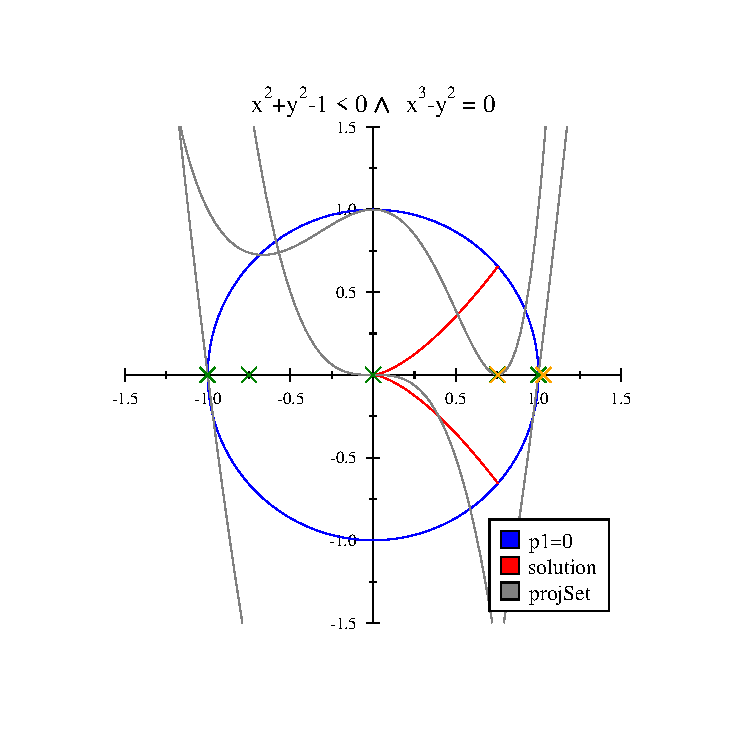
\includegraphics[scale=1.0]{cad1.eps}
%\caption{Example 1.}
%\label{fig:cad1}
%\end{figure}
% 
\begin{thebibliography}{1}
%
\bibitem{MTAA} Ralph Abraham, Jerrold E.Marsden and Tudor Ratiu.Manifolds, 
       {\em Tensor Analysis, and Applications}. Springer,
       Auflage: 2nd Corrected ed. 1988. Corr. 2nd printing 1993 edition.
%       
\bibitem{CART} Henri Cartan. {\em Differential Forms}. Dover Pubn Inc.
%
\bibitem{GMT} Herbert Federer. {\em Geometric Measure Theory}. Springer, 
       Reprint of the 1st ed. Berlin, Heidelberg, New York 1969 edition.
%
\bibitem{FLAN} Harley Flanders, {\em Differential Forms with Applications to 
       the Physical Sciences}. Dover Pubn Inc, Revised. edition.
%
\bibitem{QYBEQ} L. A. Lambe and D. E. Radford. {\em Introduction to the 
       Quantum Yang-Baxter Equation and Quantum Groups:An Algebraic Approach}.
       Springer, 1997 edition.
%
\bibitem{PMA} Walter Rudin and RudinWalter.{\em Principles of Mathematical
       Analysis}. McGraw Hill Book Co, Revised. edition.
%
\bibitem{GIT} Hassler Whitney. {\em Geometric Integration Theory}, 
       Princeton Mathematical Series, No. 21. Literary Licensing, LLC.
\end{thebibliography}
%
\end{document}
% -----------------------------------------------------------------------------
% END DOCUMENTATION
% -----------------------------------------------------------------------------
